\documentclass[10pt,UTF8]{ctexart}


\usepackage[margin=2cm,a4paper]{geometry}
%\usepackage[left=0.75in,top=0.6in,right=0.75in,bottom=1.0in,a4paper]{geometry}

\setmainfont{Caladea}
%% 也可以選用其它字庫:
% \setCJKmainfont[%
%   ItalicFont=AR PL KaitiM GB,
%   BoldFont=Noto Sans CJK SC,
% ]{Noto Serif CJK SC}
% setCJKsansfont{Noto Sans CJK SC}
% \renewcommand{\kaishu}{\CJKfontspec{AR PL KaitiM GB}}

% 繁體中文
\setCJKmainfont[Path=fonts/ ]{NotoSansTC-Medium.otf}

\usepackage{minted}
\usepackage[breaklinks]{hyperref}

% Picture
% 導言區的此三行無變化
\usepackage{graphicx}
\usepackage{float} 
\usepackage{subfigure}
% 以下是新增的自定義格式更改
\usepackage[]{caption2} %新增調用的宏包
\renewcommand{\figurename}{Fig.} %重定義編號前綴詞
\renewcommand{\captionlabeldelim}{.~} %重定義分隔符
 %\roman 是羅馬數字編號,\alph是默認的字母編號,\arabic是阿拉伯數字編號,可按需替換下一行的相應位置
\renewcommand{\thesubfigure}{(\roman{subfigure})}%此外,還可設置圖編號顯示格式,加括號或者不加括號
\makeatletter \renewcommand{\@thesubfigure}{\thesubfigure \space}%子圖編號與名稱的間隔設置
\renewcommand{\p@subfigure}{} \makeatother

% Math
\usepackage {mathtools}
\usepackage{amssymb}

% Code
\usepackage{listings}
\usepackage{xcolor}
\lstset{
    % backgroundcolor=\color{red!50!green!50!blue!50},
    % 程式碼塊背景色為淺灰色
    rulesepcolor= \color{gray}, % 程式碼塊邊框顏色
    breaklines=true,  % 程式碼過長則換行
    numbers=left, % 行號在左側顯示
    numberstyle= \small,% 行號字型
    % eywordstyle= \color{red,% 關鍵字顏色
    commentstyle=\color{gray}, % 註釋顏色
    frame=shadowbox % 用方框框住程式碼塊
    }

\usepackage{hyperref}

\title{算法分析和複雜性理論}
\author{干皓丞,2101212850, 信息工程學院}

\begin{document}
\maketitle


\section{作業目標與章節摘要}

1. LeetCode 5. Longest Palindromic Substring 最長回文子串

2. LeetCode 64. Minimum Path Sum 最小路徑和

3. LeetCode 120. Triangle, 三角形最小路徑和


\section{作業內容概述}

作業可以從 GitHub 下的 kancheng/kan-cs-report-in-2022 專案找到,作業程式碼與文件目錄為 kan-cs-report-in-2022/AATCC/lab-report/。實際執行的環境與實驗設備為 Google 的 Colab 、MacBook Pro (Retina, 15-inch, Mid 2014) 、 Acer Aspire R7 與 HP Victus (Nvidia GeForce RTX 3060)。

本作業 GitHub 專案為 kancheng/kan-cs-report-in-2022 下的 AATCC` 的目錄。程式碼可以從 code 目錄下可以找到 *.pynb,內容包含上次課堂練習、LeetCode 範例思路整理與作業。

https://github.com/kancheng/kan-cs-report-in-2022/tree/main/AATCC

\begin{figure}[H]
\centering 

\includegraphics[width=0.30\textwidth]{aatccqr.png} 
\caption{作業專案位置}
\label{Test}
\end{figure}


1. LeetCode : https://leetcode.com/

2. LeetCode CN : https://leetcode-cn.com/

3. OnlineGDB : https://www.onlinegdb.com/ 

LeetCode 的平台部分, CN 的平台有針對簡體中文使用者進行處理,包含中英文切換等功能。OnlineGDB 則可線上進行簡易的環境測試,其程式碼涵蓋 C, C++, C\#, Java, Python, JS, Rust, Go。

\newpage

\section{LeetCode 5. Longest Palindromic Substring 最長回文子串}

\subsection{LeetCode 5. 題目}

Given a string s, return the longest palindromic substring in s.

給你一個字符串 s,找到 s 中最長的回文子串。

Example 1:

\begin{lstlisting}[language={python}]
Input: s = "babad"
Output: "bab"
Explanation: "aba" is also a valid answer.
解釋:"aba" 同樣是符合題意的答案。
\end{lstlisting}

Example 2:

\begin{lstlisting}[language={python}]
Input: s = "cbbd"
Output: "bb"
\end{lstlisting}

Constraints:

1. 1 <= s.length <= 1000

2. s consist of only digits and English letters.

s 僅由數字和英文字母組成

\subsection{LeetCode 56. 思路總結}

解法一,動態規劃。定義 dp[i][j] 表示從字符串第 i 個字符到第 j 個字符這一段子串是否是回文串。由回文串的性質可以得知,回文串去掉一頭一尾相同的字符以後,剩下的還是回文串。所以狀態轉移方程是 dp[i][j] = (s[i] == s[j]) \&\& ((j-i < 3) || dp[i+1][j-1]),注意特殊的情況,j - i == 1 的時候,即只有 2 個字符的情況,只需要判斷這 2 個字符是否相同即可。 j - i == 2 的時候,即只有 3 個字符的情況,只需要判斷除去中心以外對稱的 2 個字符是否相等。每次循環動態維護保存最長回文串即可。時間複雜度 O(n\^2),空間複雜度 O(n\^2)。

解法二,中心擴散法。動態規劃的方法中,我們將任意起始,終止範圍內的字符串都判斷了一遍。其實沒有這個必要,如果不是最長回文串,無需判斷並保存結果。所以動態規劃的方法在空間複雜度上還有優化空間。判斷回文有一個核心問題是找到“軸心”。如果長度是偶數,那麼軸心是中心虛擬的,如果長度是奇數,那麼軸心正好是正中心的那個字母。中心擴散法的思想是枚舉每個軸心的位置。然後做兩次假設,假設最長回文串是偶數,那麼以虛擬中心往 2 邊擴散;假設最長回文串是奇數,那麼以正中心的字符往 2 邊擴散。擴散的過程就是對稱判斷兩邊字符是否相等的過程。這個方法時間複雜度和動態規劃是一樣的,但是空間複雜度降低了。時間複雜度 O(n\^2),空間複雜度 O(1)。

解法三,滑動窗口。這個寫法其實就是中心擴散法變了一個寫法。中心擴散是依次枚舉每一個軸心。滑動窗口的方法稍微優化了一點,有些軸心兩邊字符不相等,下次就不會枚舉這些不可能形成回文子串的軸心了。不過這點優化並沒有優化時間複雜度,時間複雜度 O(n\^2),空間複雜度 O(1)。

解法四,馬拉車算法。這個算法是本題的最優解,也是最複雜的解法。時間複雜度 O(n),空間複雜度 O(n)。中心擴散法有 2 處有重複判斷,第一處是每次都往兩邊擴散,不同中心擴散多次,實際上有很多重複判斷的字符,能否不重複判斷?第二處,中心能否跳躍選擇,不是每次都枚舉,是否可以利用前一次的信息,跳躍選擇下一次的中心?馬拉車算法針對重複判斷的問題做了優化,增加了一個輔助數組,將時間複雜度從 O(n\^2) 優化到了 O(n),空間換了時間,空間複雜度增加到 O(n)。

https://books.halfrost.com/leetcode/ChapterFour/0001~0099/0005.Longest-Palindromic-Substring/

\subsection{LeetCode 5. Code 範例}

LeetCode 5. Python 

\begin{lstlisting}[language={python}]
class Solution:
    def longestPalindrome(self, s: str) -> str:
        if s == s[::-1]:
            return s
        max_len = 1
        ans = s[0]
        for i in range(1, len(s)):
            if i - max_len - 1 >= 0 and s[i - max_len - 1: i + 1] == s[i - max_len - 1: i + 1][::-1]:
                ans = s[i - max_len - 1: i + 1]
                max_len += 2
            if i - max_len >= 0 and s[i - max_len: i + 1] == s[i - max_len: i + 1][::-1]:
                ans = s[i - max_len: i + 1]
                max_len += 1
        return ans
\end{lstlisting}

\subsection{LeetCode 5. 結果}

\begin{figure}[H]
\centering 
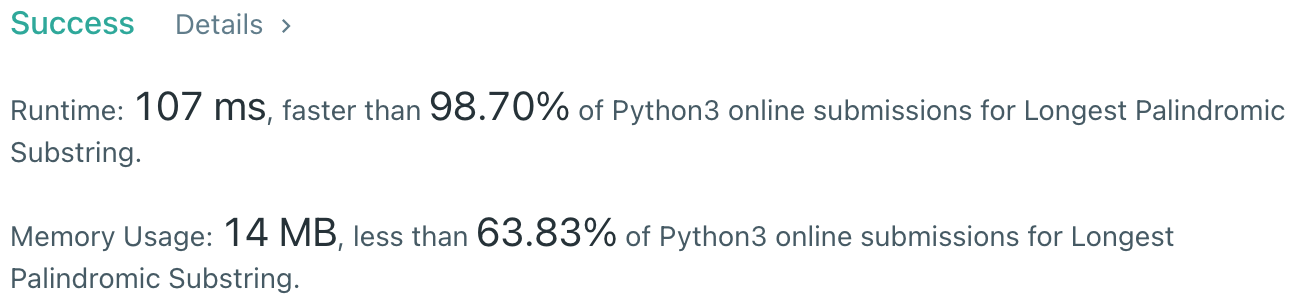
\includegraphics[width=0.80\textwidth]{lc-5-o.png} 
\caption{LeetCode 5 結果}
\label{Test}
\end{figure}


\newpage

\section{LeetCode 64. Minimum Path Sum 最小路徑和}

\subsection{LeetCode 64. 題目}

Given a m x n grid filled with non-negative numbers, find a path from top left to bottom right, which minimizes the sum of all numbers along its path.

Note: You can only move either down or right at any point in time.


給定一個包含非負整數的 m x n 網格 grid ,請找出一條從左上角到右下角的路徑,使得路徑上的數字總和為最小。

說明:每次只能向下或者向右移動一步。

\begin{figure}[H]
\centering 
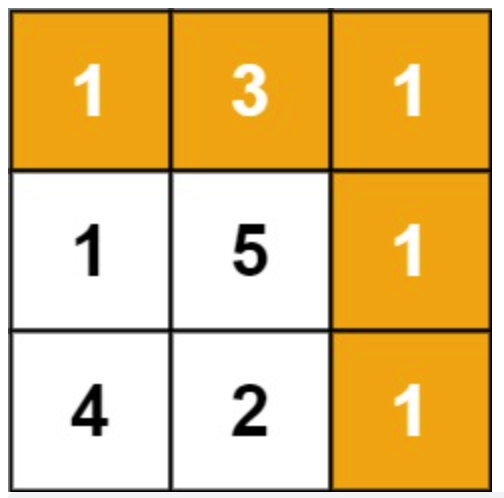
\includegraphics[width=0.40\textwidth]{lc-64-p-example.png} 
\caption{Example}
\label{Test}
\end{figure}

Example 1:

\begin{lstlisting}[language={python}]
Input: grid = [[1,3,1],[1,5,1],[4,2,1]]
Output: 7
Explanation: Because the path 1 → 3 → 1 → 1 → 1 minimizes the sum.
因為路徑 1→3→1→1→1 的總和最小。
\end{lstlisting}

Example 2:

\begin{lstlisting}[language={python}]
Input: grid = [[1,2,3],[4,5,6]]
Output: 12
\end{lstlisting}

Constraints:

1. m == grid.length

2. n == grid[i].length

3. 1 <= m, n <= 200

4. 0 <= grid[i][j] <= 100

\subsection{LeetCode 64. 思路總結}

1. 給定一個包含非負整數的 m x n 網格,請找出一條從左上角到右下角的路徑,使得路徑上的數字總和為最小。說明:每次只能向下或者向右移動一步。

2. 在地圖上求出從左上角到右下角的路徑中,數字之和最小的一個,輸出數字和。

3. 這一題最簡單的想法就是用一個二維數組來 DP,當然這是最原始的做法。由於只能往下和往右走,只需要維護 2 列信息就可以了,從左邊推到最右邊即可得到最小的解。

\subsection{LeetCode 64. Code 範例}

\begin{lstlisting}[language={python}]
class Solution(object):
    def minPathSum(self, grid):
        #此數組用於記憶化搜索
        dp = [[0]*len(grid[0]) for i in range(len(grid))]
        for i in range(len(grid)):
            for j in range(len(grid[0])):
                #在起點的時候
                if (i == 0 and j == 0):
                    dp[i][j] = grid[0][0]
                #在左邊緣的時候
                elif (j == 0 and i != 0):
                    dp[i][j] = dp[i - 1][j]  + grid[i][j]
                #在上邊緣的時候
                elif (i == 0 and j != 0):
                    dp[i][j] = dp[i][j-1] + grid[i][j]
                # 普遍情況下
                else:
                    dp[i][j] = min(dp[i - 1][j], dp[i][j - 1]) + grid[i][j]                    
        return dp[len(grid)-1][len(grid[0])-1]
\end{lstlisting}

\subsection{LeetCode 64. 結果}

\begin{figure}[H]
\centering 
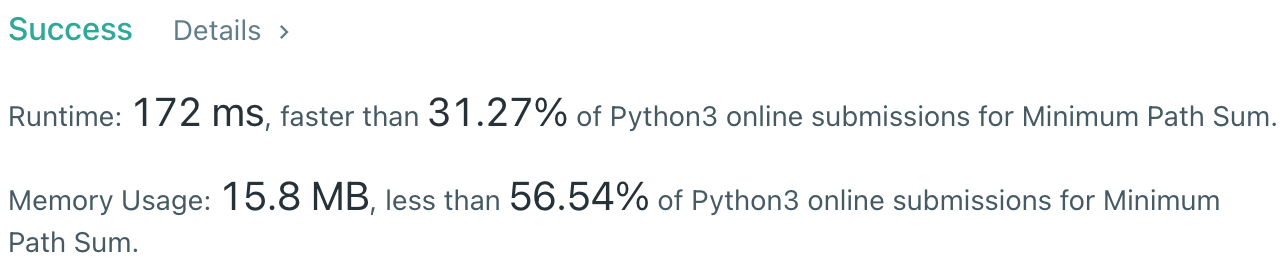
\includegraphics[width=0.80\textwidth]{lc-64-o.png} 
\caption{LeetCode 64 結果}
\label{Test}
\end{figure}


\newpage

\section{LeetCode 120. Triangle, 三角形最小路徑和}

\subsection{LeetCode 120. 題目}

Given a triangle array, return the minimum path sum from top to bottom.

For each step, you may move to an adjacent number of the row below. More formally, if you are on index i on the current row, you may move to either index i or index i + 1 on the next row.

給定一個三角形 triangle ,找出自頂向下的最小路徑和。

每一步只能移動到下一行中相鄰的結點上。相鄰的結點 在這裡指的是 下標 與 上一層結點下標 相同或者等於 上一層結點下標 + 1 的兩個結點。也就是說,如果正位於當前行的下標 i ,那麼下一步可以移動到下一行的下標 i 或 i + 1 。

Example 1:

\begin{lstlisting}[language={python}]
Input: triangle = [[2],[3,4],[6,5,7],[4,1,8,3]]
Output: 11
Explanation: The triangle looks like:
   2
  3 4
 6 5 7
4 1 8 3
The minimum path sum from top to bottom is 2 + 3 + 5 + 1 = 11 (underlined above).
自頂向下的最小路徑和為 11(即,2 + 3 + 5 + 1 = 11)。
\end{lstlisting}

Example 2:
\begin{lstlisting}[language={python}]
Input: triangle = [[-10]]
Output: -10
\end{lstlisting}

Constraints:

1. 1 <= triangle.length <= 200

2. triangle[0].length == 1

3. triangle[i].length == triangle[i - 1].length + 1

4. $-10^{4} <= triangle[i][j] <= 10^{4}$

Follow up: Could you do this using only O(n) extra space, where n is the total number of rows in the triangle?
你可以只使用 O(n) 的額外空間(n 為三角形的總行數)來解決這個問題嗎?

\subsection{LeetCode 120. 思路總結}

1. 求出從三角形頂端到底端的最小和。要求最好用 O(n) 的時間複雜度。

2. 這一題最優解是不用輔助空間,直接從下層往上層推。普通解法是用二維數組 DP,稍微優化的解法是一維數組 DP。

\subsection{LeetCode 120. Code 範例}

\begin{lstlisting}[language={python}]
from typing import List
class Solution:
    def minimumTotal(self, triangle: List[List[int]]) -> int:
        depth = len(triangle)
        for i in range(-2, -depth-1, -1):
            for j in range(depth + 1 + i):
                triangle[i][j] += min(triangle[i+1][j], triangle[i+1][j+1])
        return triangle[0][0]
\end{lstlisting}

\subsection{LeetCode 120. 結果}

\begin{figure}[H]
\centering 
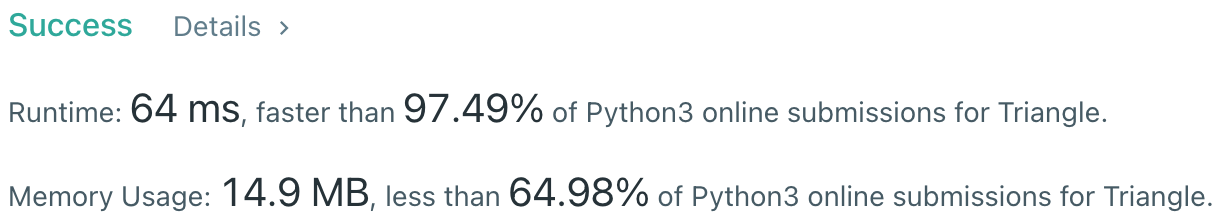
\includegraphics[width=0.80\textwidth]{lc-120-o.png} 
\caption{LeetCode 120 結果}
\label{Test}
\end{figure}




%\section{附錄}

% 數學意義說明

% $$\min \limits_{G}\max \limits_{D}{V_I(D,\ G)=V(D,G)-\lambda L_I(G,Q)}$$

%	\begin{lstlisting}[language={python}]

%	\end{lstlisting}

%\begin{enumerate}
%\item Y
%\item A
%\end{enumerate}

% \newpage

\clearpage

\end{document}